\section{Essentials}
This section will cover the essentials in order to get started. 
\subsection{The set of Real numbers}
\begin{itemize}
    \item $\mathbb{N} = \{1, 2, 3, ...\}$ - - The set of natural numbers. 
    \item $\mathbb{Z} = \{..., -2, -1, 0, 1, 2, ...\}$ - The set of integers.
    \item $\mathbb{Q} = \{\frac{a}{b} | a, b \in \mathbb{Z}, b \neq 0\}$ - The set of rational numbers. 
    \item $\mathbb{I}$ - The set of Irrational Numbers(Real numbers that are not rational). 
    \item $\mathbb{R} = \mathbb{Q} \cup \mathbb{I}$
\end{itemize}


\subsection{The properties of Real numbers}
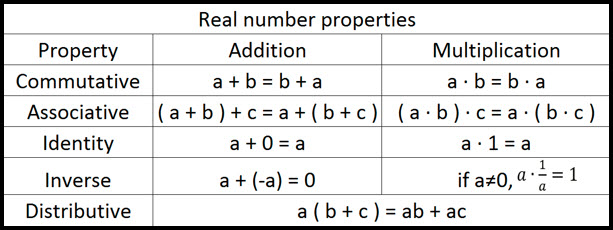
\includegraphics{algebra-pre-calculus/essentials/sets2.jpg}
\begin{itemize}
    \item The associative property of addition states that you can group the addends in different ways without changing the outcome. The commutative property of addition states that you can reorder the addends without changing the outcome.
    \item The commutative property of multiplication shows that it is acceptable to rearrange terms when multiplying. In contrast, the associative property of multiplication moves parentheses to order the multiplication.
    \item According to the distributive property, multiplying the sum of two or more addends by a number will give the same result as multiplying each addend individually by the number and then adding the products together.
    \item The multiplicative inverse property states that if we multiply a number with its reciprocal, the product is always equal to 1.
    \item The inverse property of addition states that adding a number and it's opposite, called the additive inverse, will produce a sum of zero.
\end{itemize}
